
\documentclass[a4paper, 10pt, twoside]{article}

\usepackage[top=1in, bottom=1in, left=1in, right=1in]{geometry}
\usepackage[utf8]{inputenc}
\usepackage[spanish, es-ucroman, es-noquoting]{babel}
\usepackage{setspace}
\usepackage{fancyhdr}
\usepackage{lastpage}
\usepackage{amsmath}
\usepackage{amsfonts}
\usepackage{amsthm}
\usepackage{verbatim}
\usepackage{fancyvrb}
\usepackage{graphicx}
\usepackage{float}
\usepackage{enumitem} % Provee macro \setlist
\usepackage{tabularx}
\usepackage{multirow}
\usepackage{hyperref}
\usepackage{xspace}
\usepackage{ulem} % Provee macro \uwave
\usepackage[toc, page]{appendix}


%%%%%%%%%% Constantes - Inicio %%%%%%%%%%
\newcommand{\titulo}{Trabajo Práctico 1}
\newcommand{\materia}{Bases de Datos}
\newcommand{\integrantes}{Hosen · Caravario · Rajgnewerc · Russo}
\newcommand{\cuatrimestre}{Primer Cuatrimestre de 2016}
%%%%%%%%%% Constantes - Fin %%%%%%%%%%


%%%%%%%%%% Configuración de Fancyhdr - Inicio %%%%%%%%%%
\pagestyle{fancy}
\thispagestyle{fancy}
\lhead{\titulo · \materia}
\rhead{\integrantes}
\renewcommand{\footrulewidth}{0.4pt}
\cfoot{\thepage /\pageref{LastPage}}

\fancypagestyle{caratula} {
   \fancyhf{}
   \cfoot{\thepage /\pageref{LastPage}}
   \renewcommand{\headrulewidth}{0pt}
   \renewcommand{\footrulewidth}{0pt}
}
%%%%%%%%%% Configuración de Fancyhdr - Fin %%%%%%%%%%


%%%%%%%%%% Miscelánea - Inicio %%%%%%%%%%
% Evita que el documento se estire verticalmente para ocupar el espacio vacío
% en cada página.
\raggedbottom

% Separación entre párrafos.
\setlength{\parskip}{0.5em}

% Separación entre elementos de listas.
\setlist{itemsep=0.5em}

% Asigna la traducción de la palabra 'Appendices'.
\renewcommand{\appendixtocname}{Apéndices}
\renewcommand{\appendixpagename}{Apéndices}
%%%%%%%%%% Miscelánea - Fin %%%%%%%%%%


%%%%%%%%%% Macros para el modelo relacional - Inicio %%%%%%%%%%
\newcommand{\relacion}[3]{
  \noindent
  \textbf{#1}(\ignorespaces#2\unskip) \\
  #3
  \vspace{0.5em}
}
\newcommand{\pk}[1]{%
  \underline{#1}%
}
\newcommand{\fk}[1]{%
  \uwave{#1}%
}
\newcommand{\pkfk}[1]{%
  \pk{\fk{#1}}%
}
\newcommand{\clavespkck}[1]{
  PK = CK = \{#1\}
}
\newcommand{\clavespkckfk}[1]{
  PK = CK = FK = \{#1\}
}
\newcommand{\clavesfk}[1]{
  FK = \{#1\}
}
%%%%%%%%%% Macros para el modelo relacional - Fin %%%%%%%%%%

\begin{document}


%%%%%%%%%%%%%%%%%%%%%%%%%%%%%%%%%%%%%%%%%%%%%%%%%%%%%%%%%%%%%%%%%%%%%%%%%%%%%%%
%% Carátula                                                                  %%
%%%%%%%%%%%%%%%%%%%%%%%%%%%%%%%%%%%%%%%%%%%%%%%%%%%%%%%%%%%%%%%%%%%%%%%%%%%%%%%


\thispagestyle{caratula}

\begin{center}


\includegraphics[height=2cm]{DC.png} 
\hfill

\includegraphics[height=2cm]{UBA.jpg} 

\vspace{2cm}

Departamento de Computación,\\
Facultad de Ciencias Exactas y Naturales,\\
Universidad de Buenos Aires

\vspace{4cm}

\begin{Huge}
\titulo
\end{Huge}

\vspace{0.5cm}

\begin{Large}
\materia
\end{Large}

\vspace{1cm}

\cuatrimestre

\vspace{4cm}

\begin{tabular}{|c|c|c|}
\hline
Apellido y Nombre & LU & E-mail\\
\hline
Federico Hosen  & 825/12 & federico.hosen@gmail.com\\
Martin Caravario  & 470/12 & martin.caravario@gmail.com\\
Guido Rajgnewerc  & 379/12 & guido.raj@gmail.com\\
Christian Russo  & 679/10 & christian.russo8@gmail.com\\
\hline
\end{tabular}

\end{center}

\newpage


%%%%%%%%%%%%%%%%%%%%%%%%%%%%%%%%%%%%%%%%%%%%%%%%%%%%%%%%%%%%%%%%%%%%%%%%%%%%%%%
%% Introducción                                                              %%
%%%%%%%%%%%%%%%%%%%%%%%%%%%%%%%%%%%%%%%%%%%%%%%%%%%%%%%%%%%%%%%%%%%%%%%%%%%%%%%


\section{Introducción}

Presentaremos una soluci\'on para el problema de un \textbf{Mercado Virtual} tomando como gu\'ia el \textbf{Khan El-Khalili} ubicado en El Cairo, Egipto. El problema en cuesti\'on contempla una serie de restricciones sobre como se realizan la compra y venta de productos por internet. Cada publicaci\'on puede tener distintos tipos y ser de distintas formas, haciendo que esto impacte en la facturaci\'on del usuario que publica. Por otro lado se cuenta con un sistema de comentarios y calificaciones.

Utilizaremos las herramientas vistas en la materia, el modelado basado en el Diagrama de Entidad Relaci\'on, su MR resultante y la base de datos final que presentaremos en MySQL.

%%%%%%%%%%%%%%%%%%%%%%%%%%%%%%%%%%%%%%%%%%%%%%%%%%%%%%%%%%%%%%%%%%%%%%%%%%%%%%%
%% Diagrama de Entidad Relación                                              %%
%%%%%%%%%%%%%%%%%%%%%%%%%%%%%%%%%%%%%%%%%%%%%%%%%%%%%%%%%%%%%%%%%%%%%%%%%%%%%%%


\section{Diagrama de Entidad Relación}

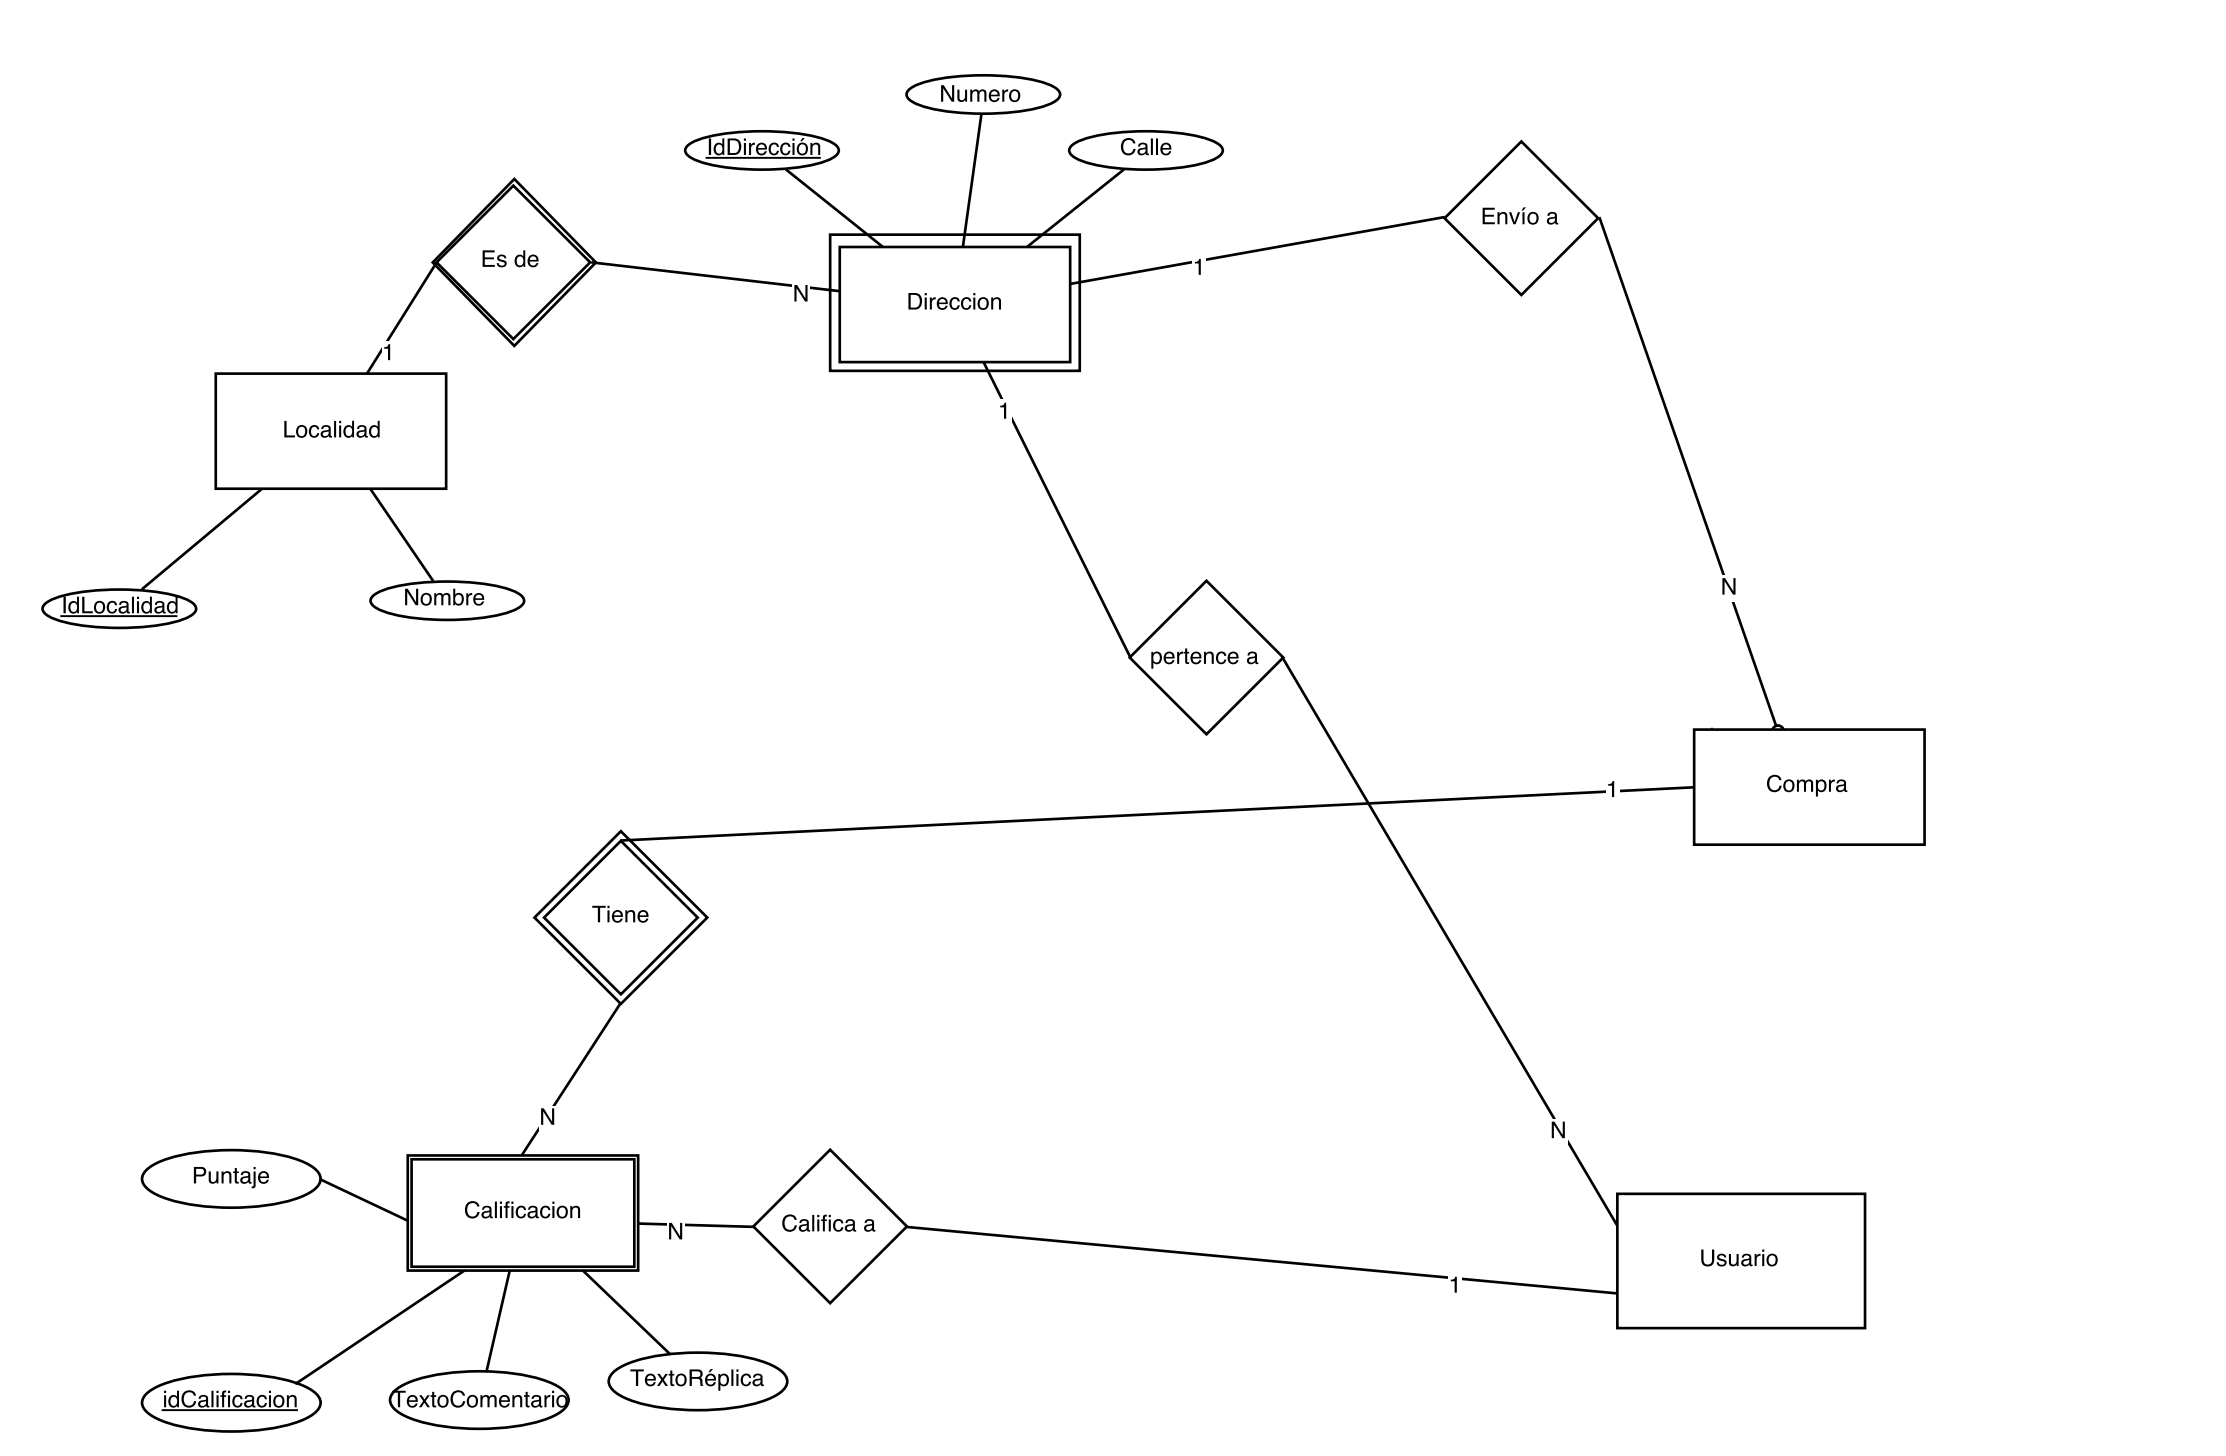
\includegraphics[width=20cm, height=12cm]{der1}
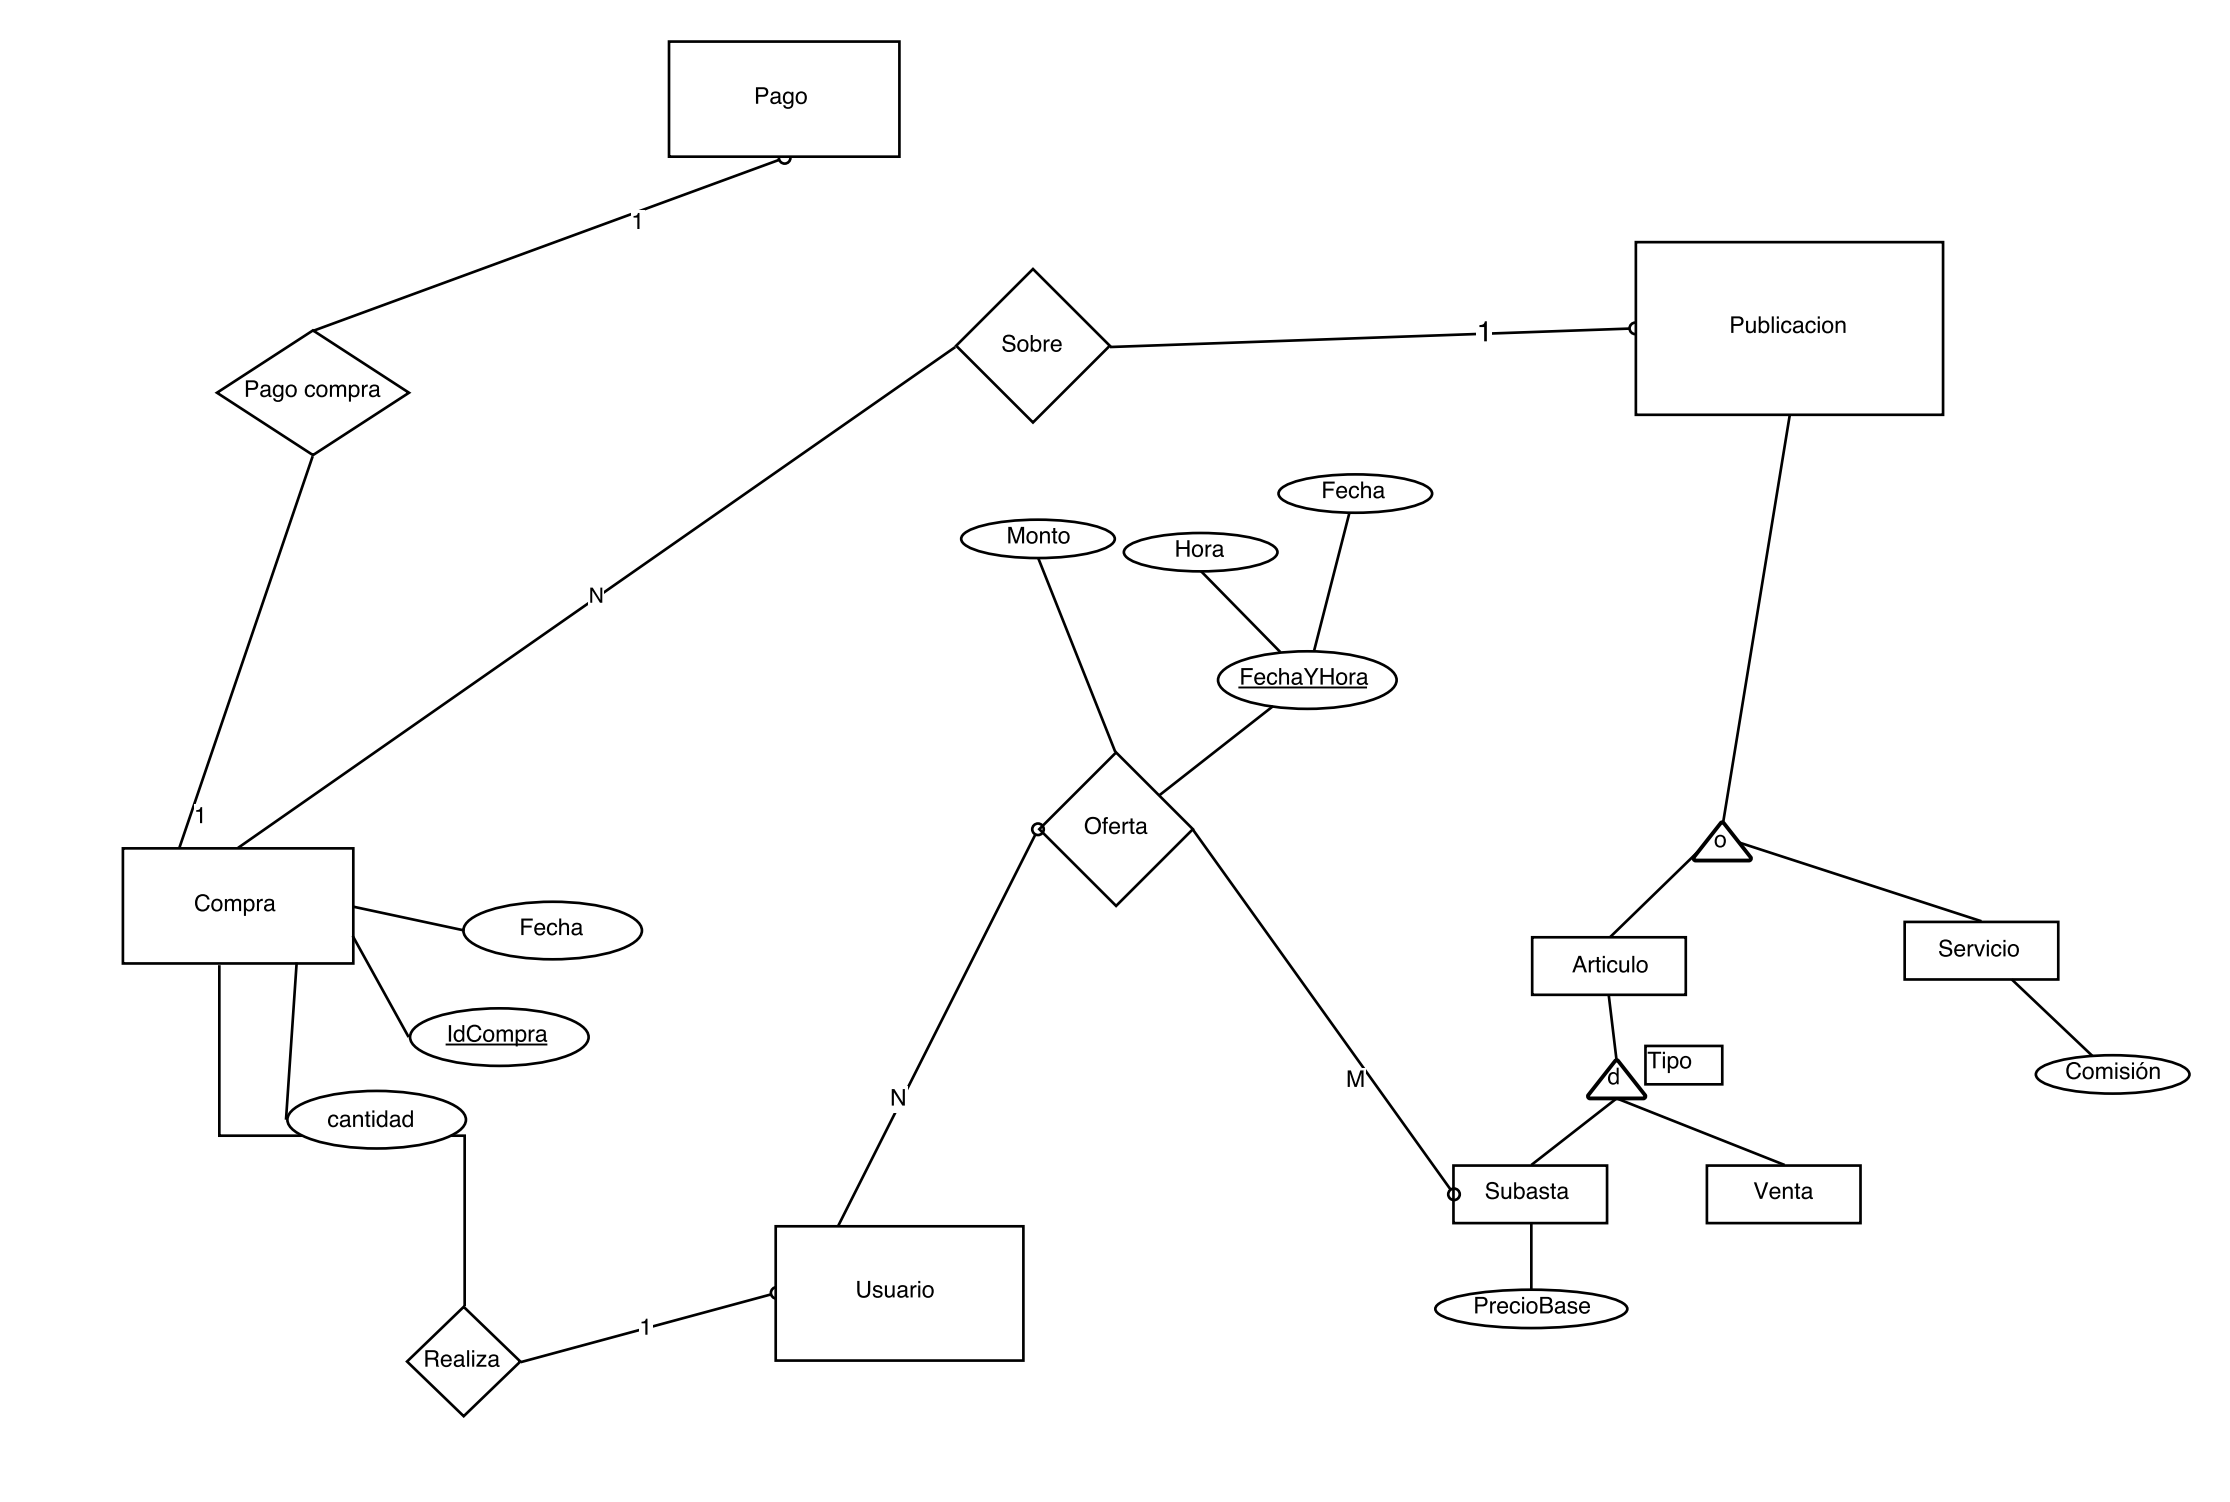
\includegraphics[width=18cm, height=12cm]{der2}
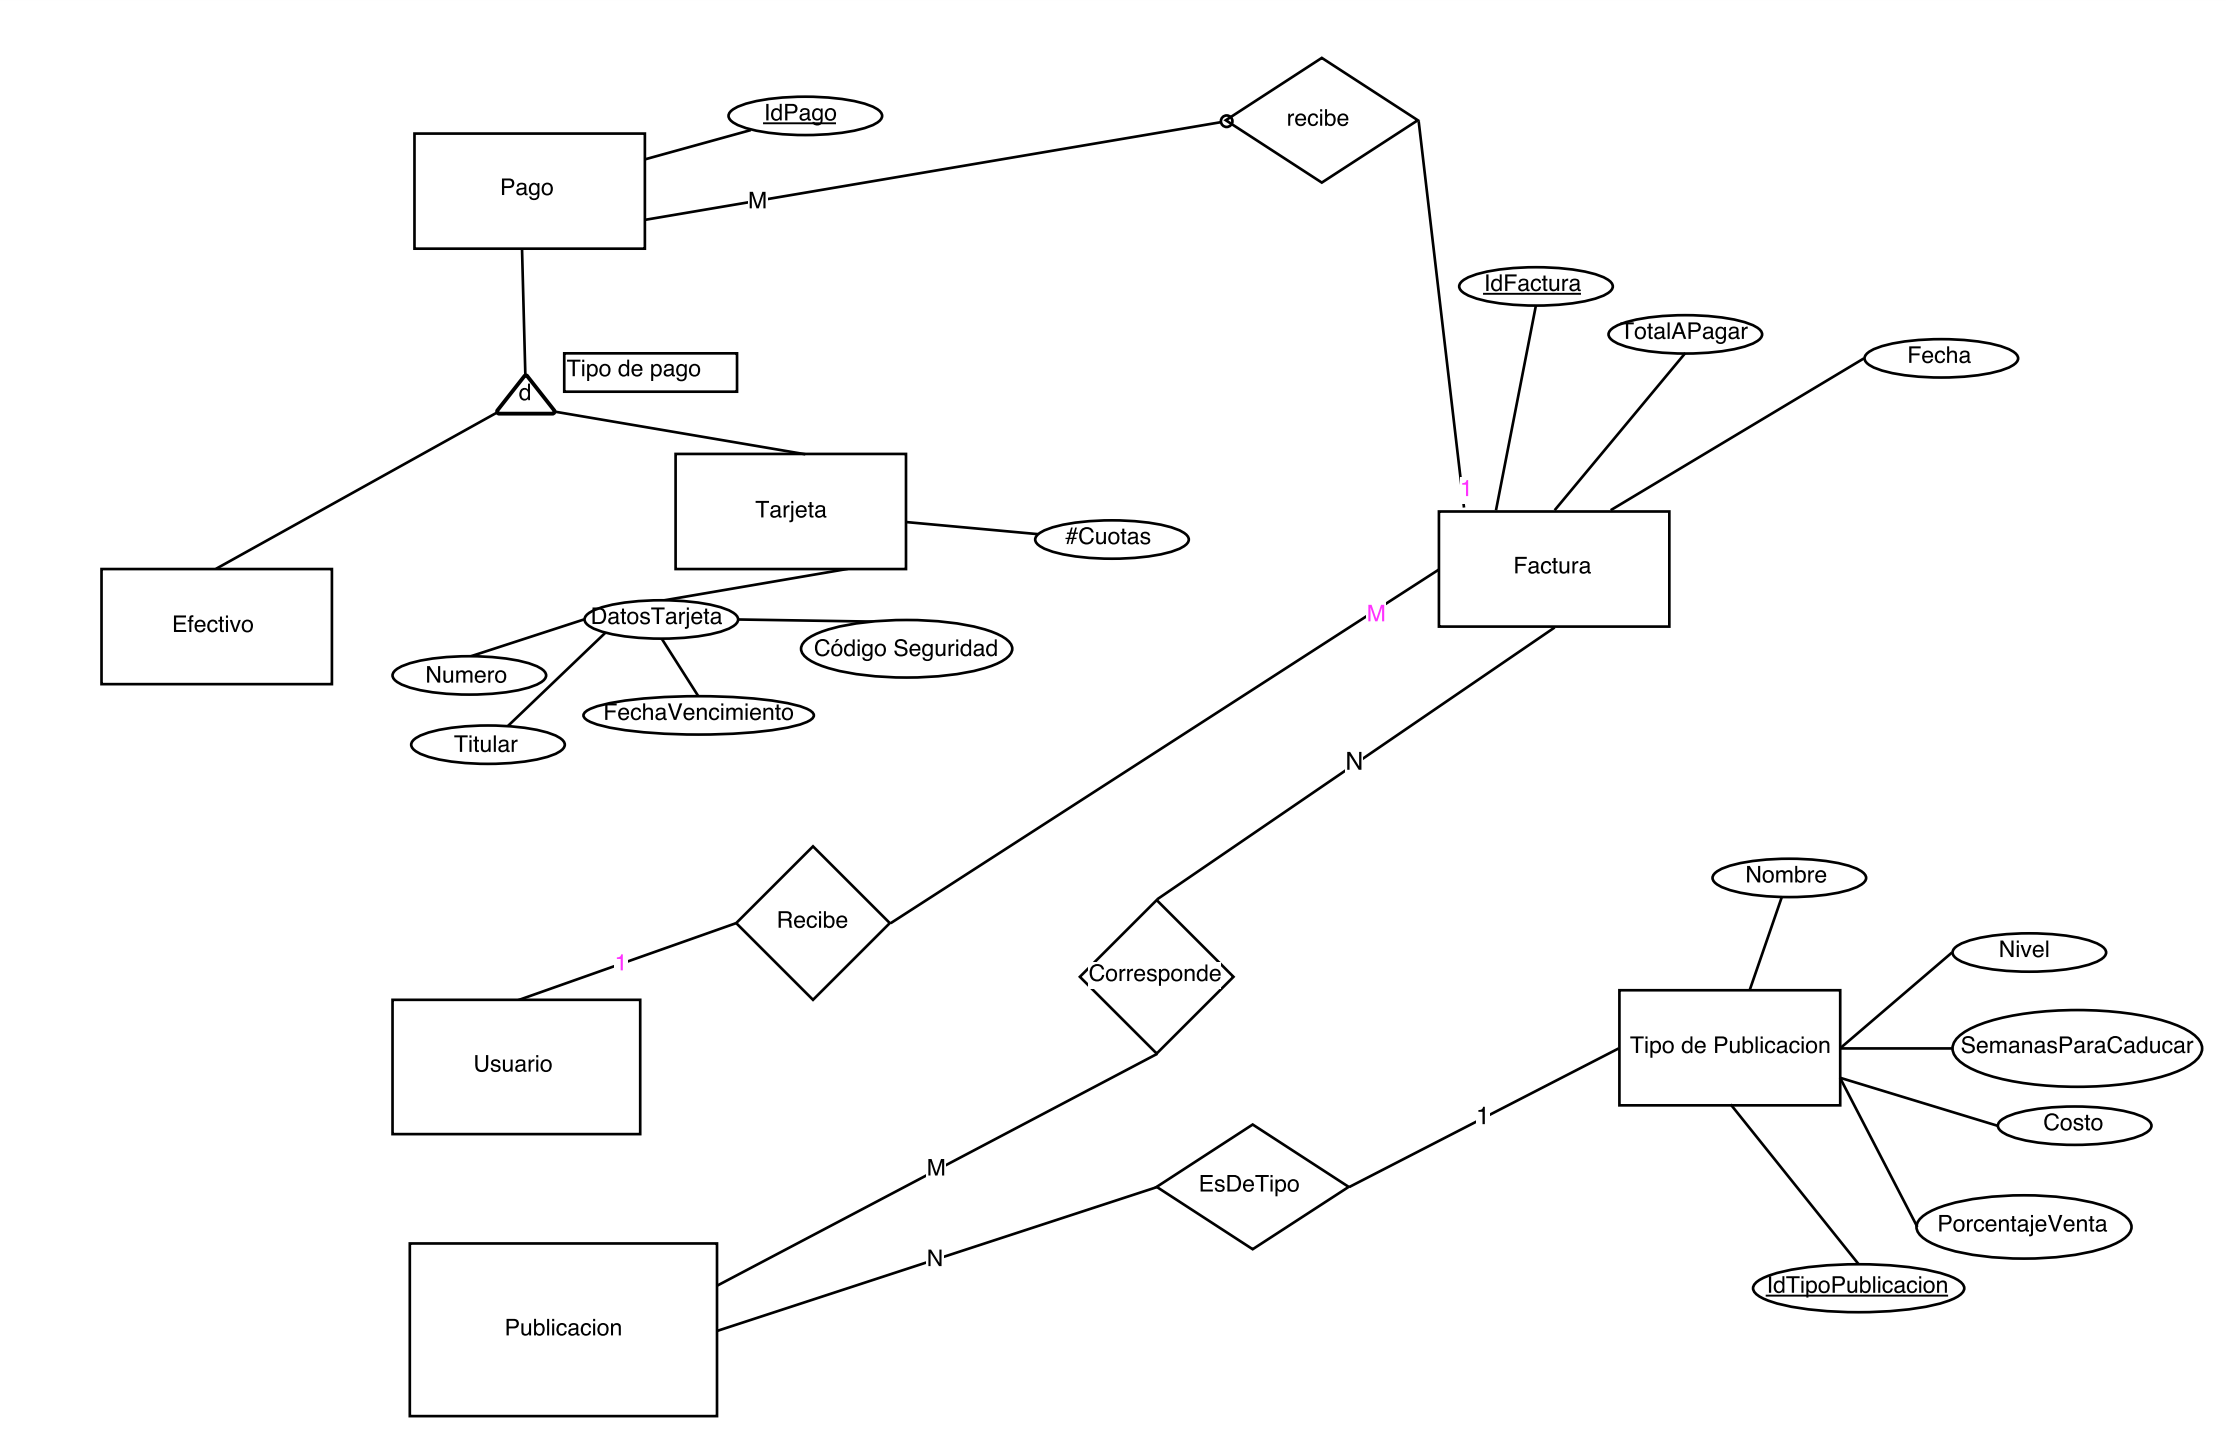
\includegraphics[width=18cm, height=12cm]{der3}
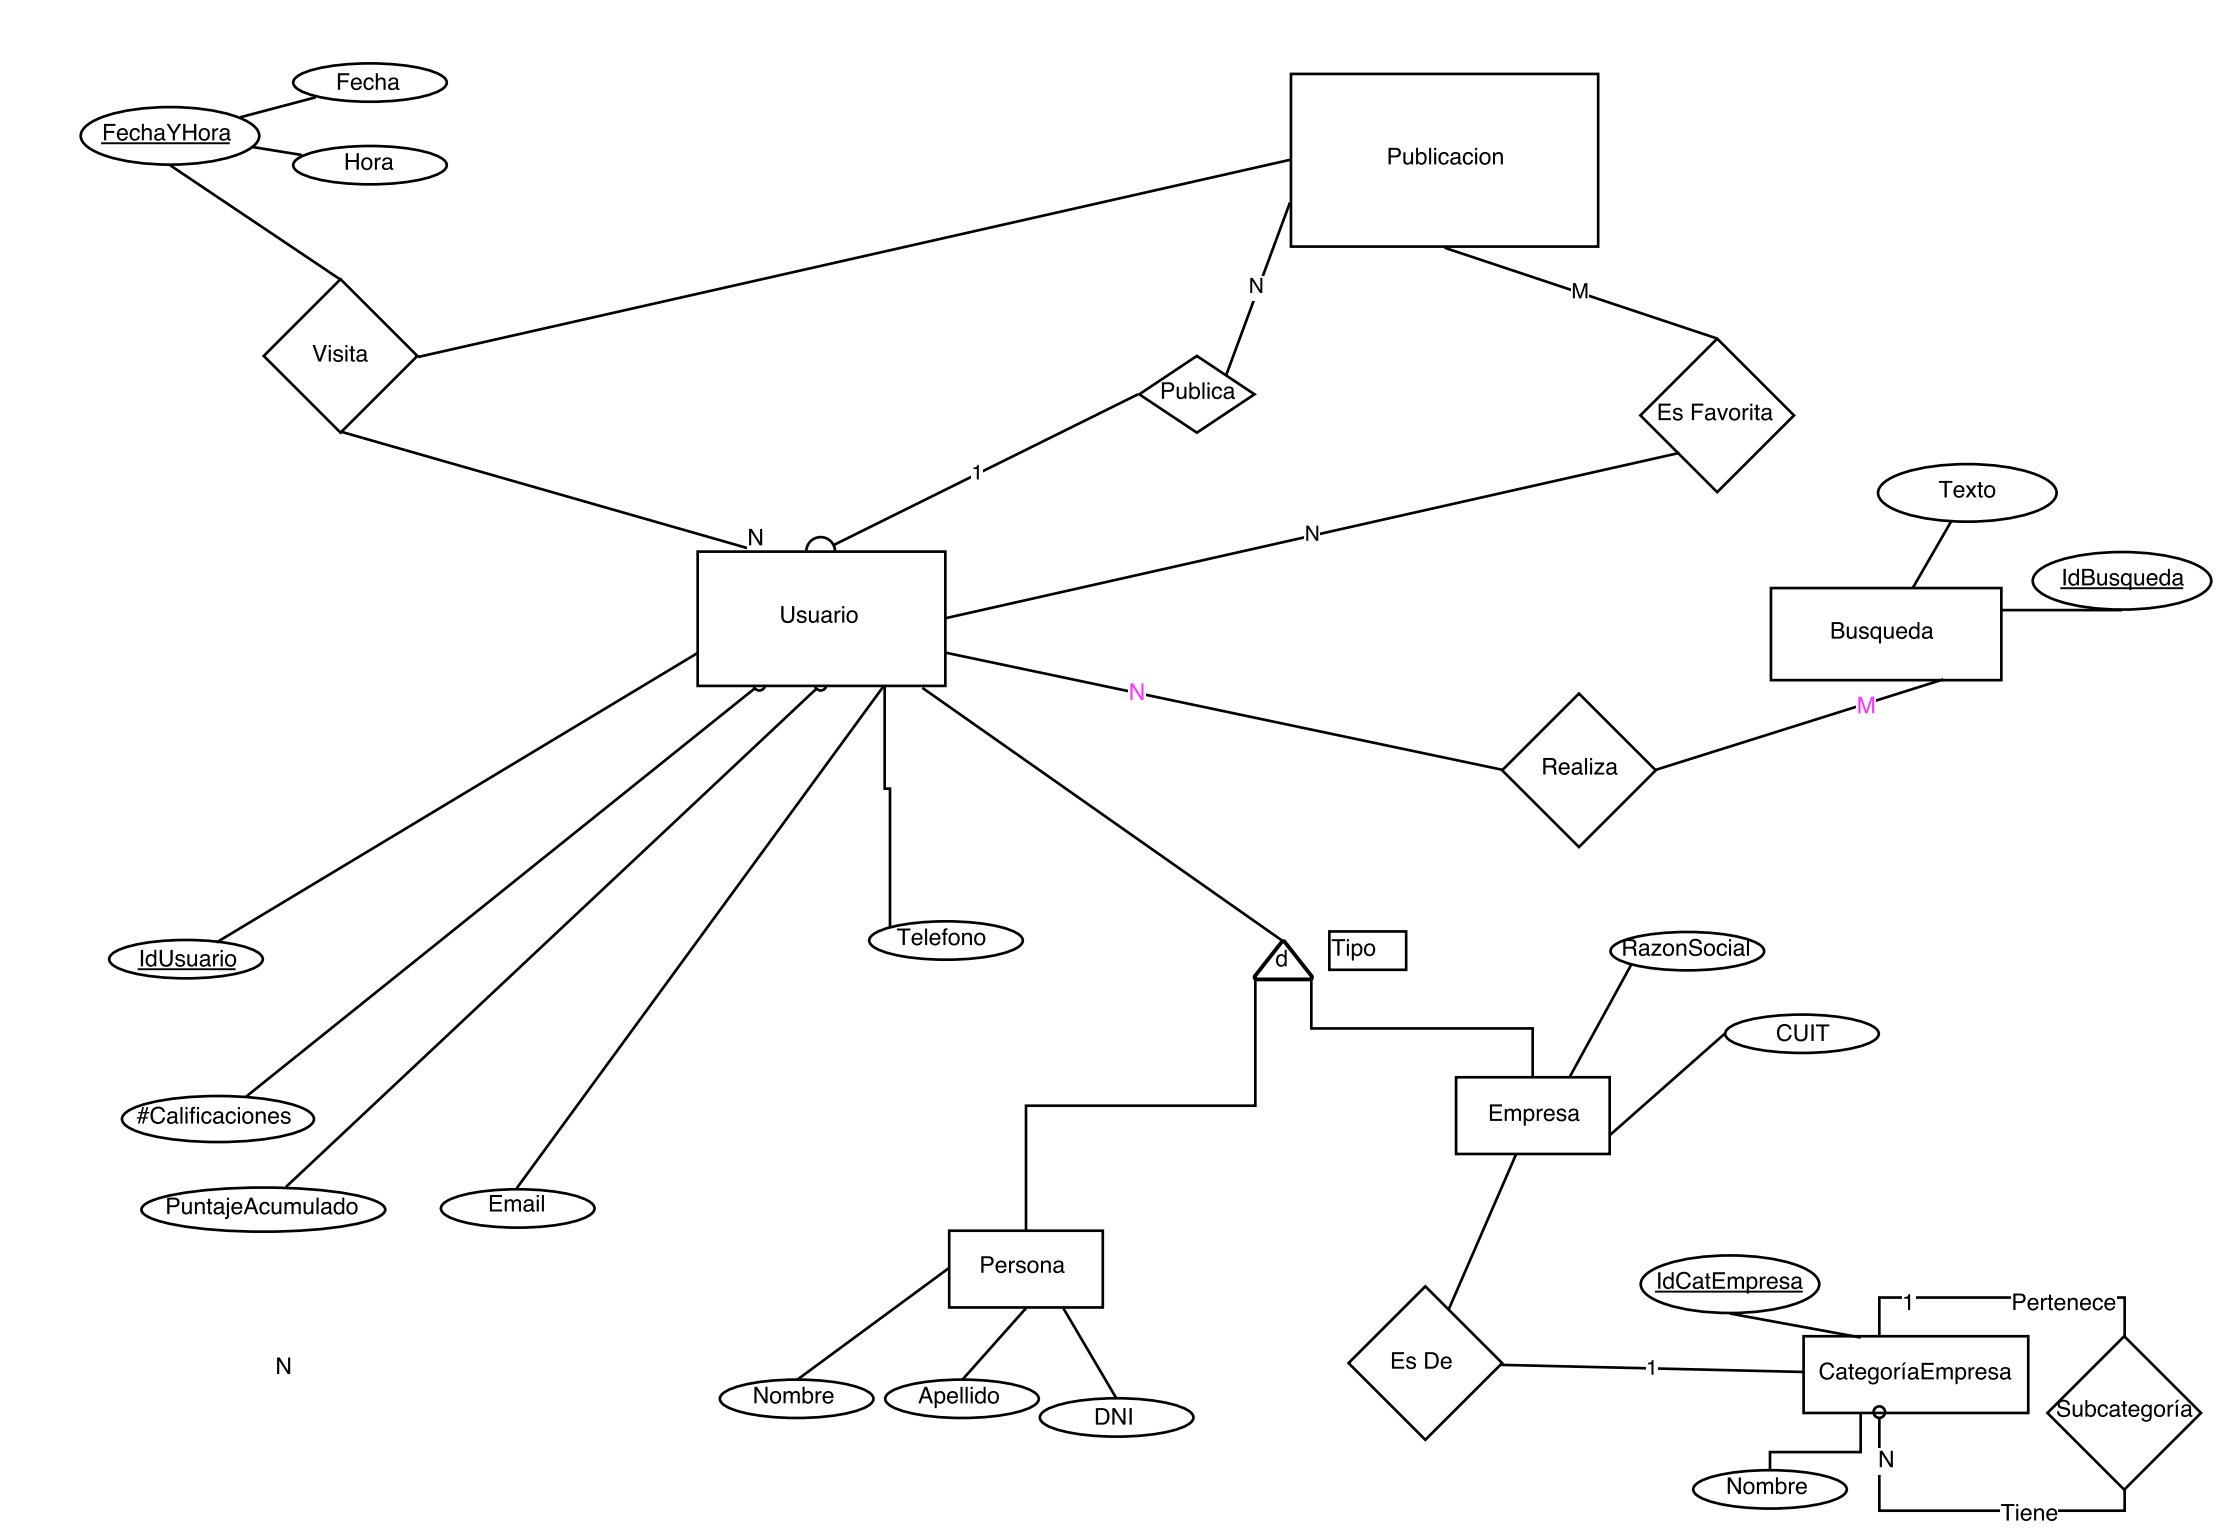
\includegraphics[width=18cm, height=12cm]{der4}
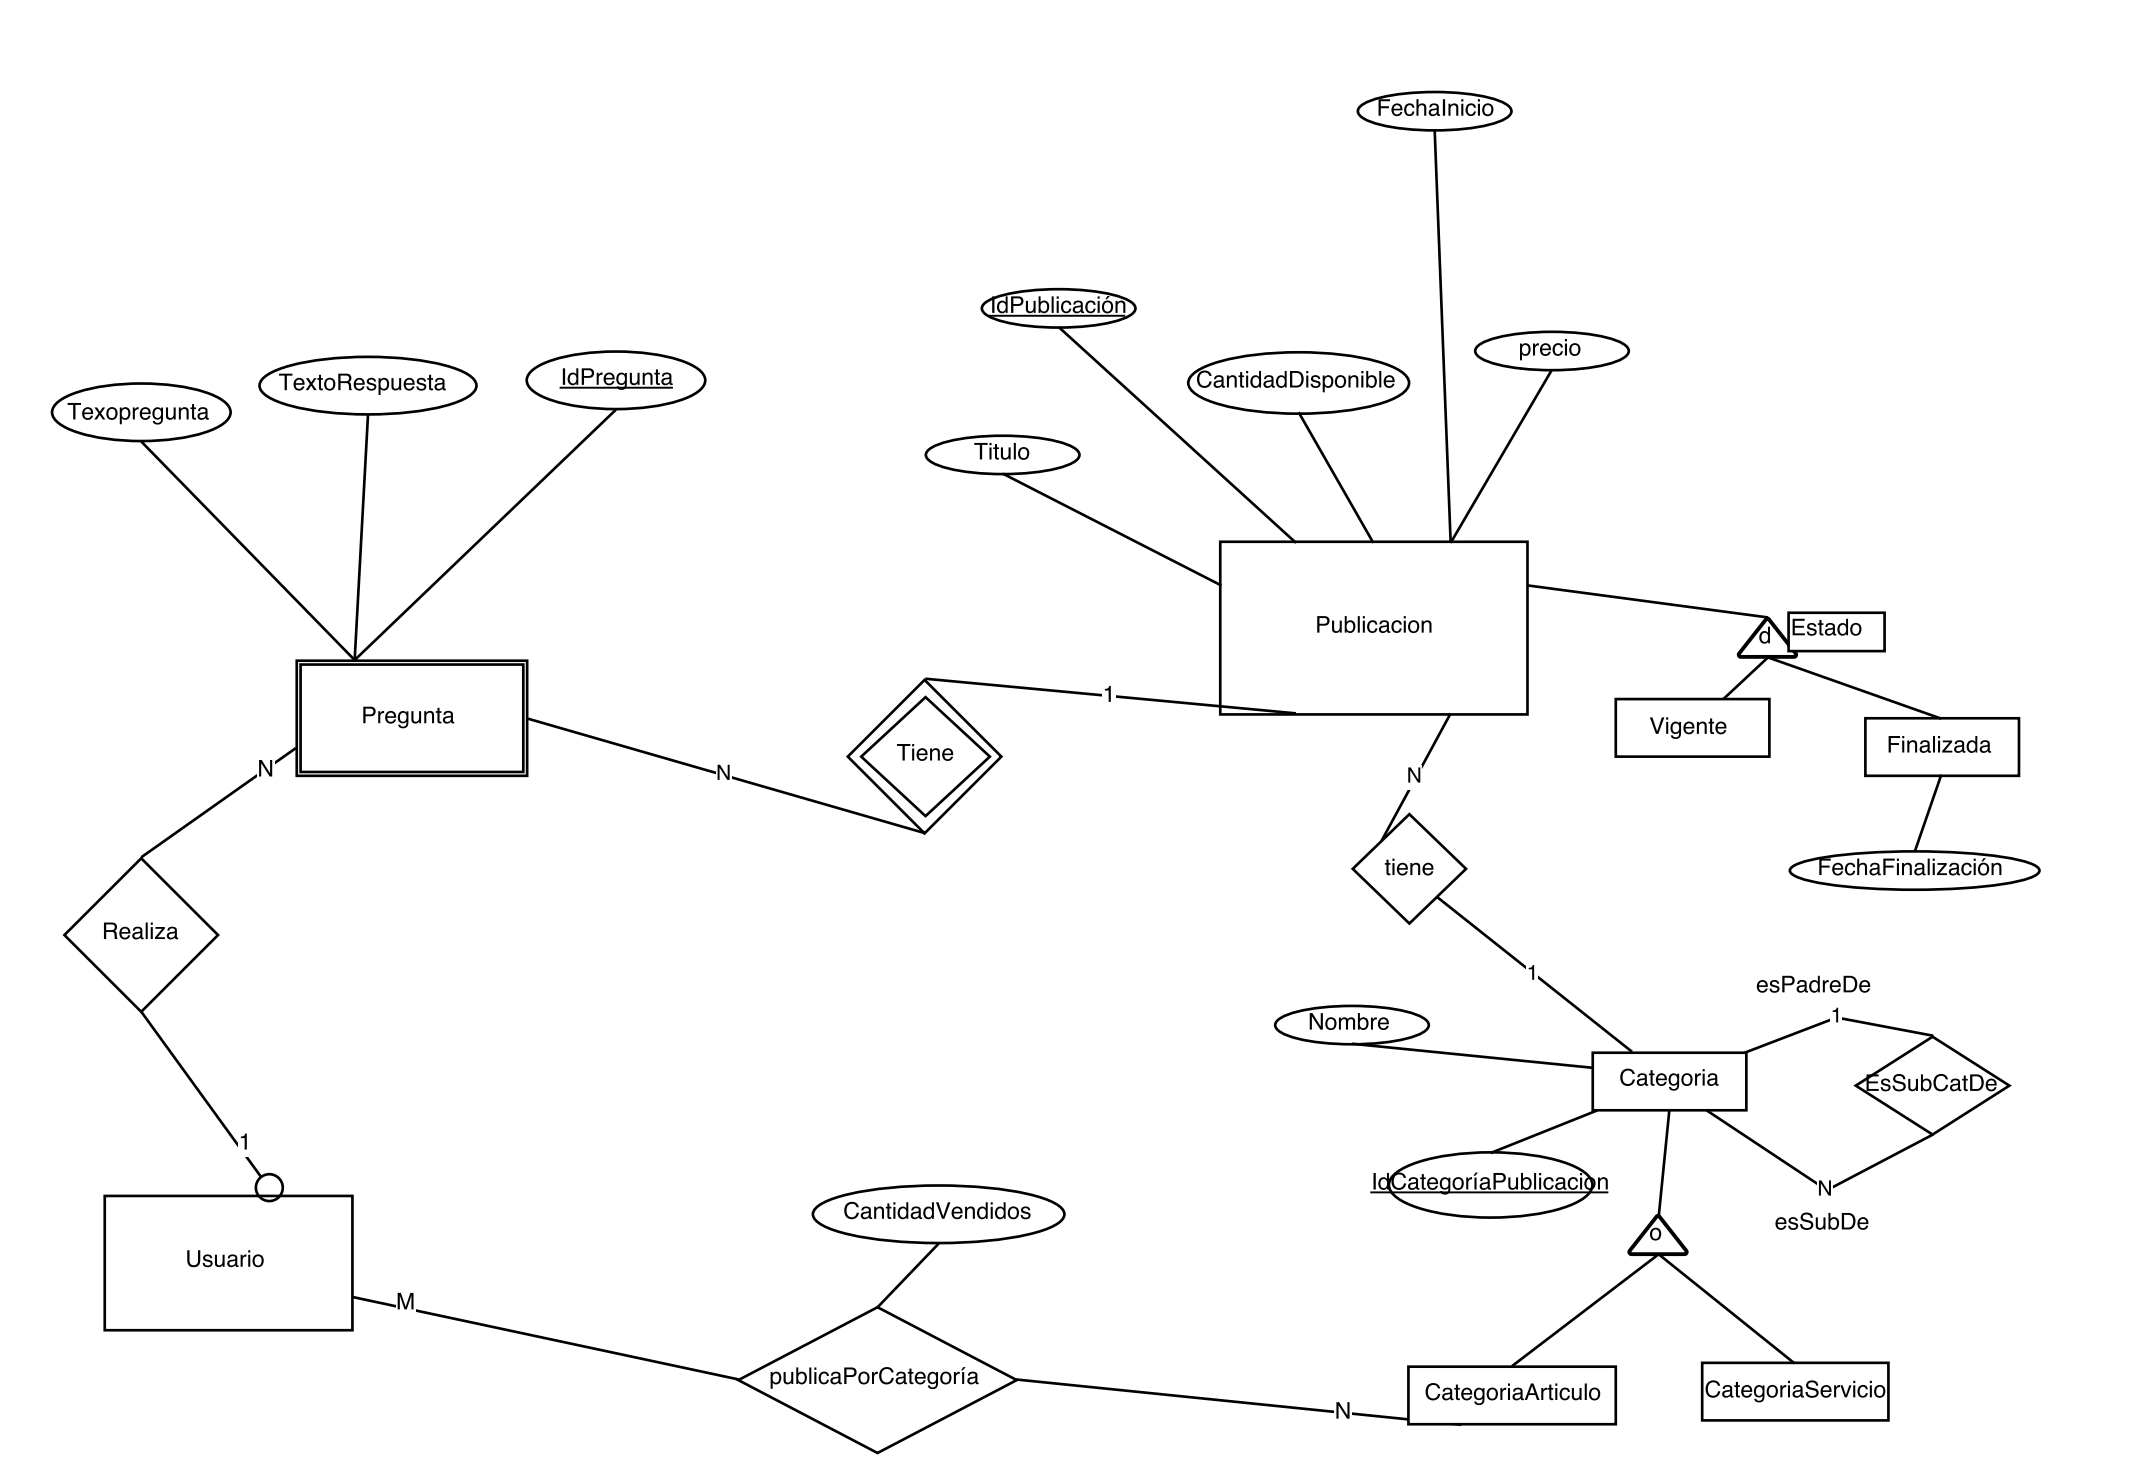
\includegraphics[width=19cm, height=12cm]{der5}

\subsection{Restricciones}

\begin{enumerate}
\item No puede haber dos DNI iguales. 
\item La publicaci\'on del tipo Libre! tiene costo 0.
\item Para cada compraventa existen a lo sumo 2 calificaciones, cada una correspondiente al comprador y vendedor.
\item El nivel de la publicaci\'on es distinto para cada tipo de publicaci\'on.
\item El usuario que compra una publicaci\'on no puede ser el usuario que publica.
\item Si un usuario realiza una respuesta a un comentario, entonces dicho comentario es de una calificaci\'on y la calificaci\'on fue hecha por un usuario que hizo dicha  compra 
\item Las publicaciones del tipo Rub\'iDelOriente aparecen primeras en las b\'usquedas. Luego aparecen en orden de mayor a menor costo de comisi\'on y por \'ultimo las de la categor\'ia Libre!.
\item El costo por mes de Rub\'iDeOriente es Fijo y se pueden hacer 3 publicaciones por mes de este tipo usuario.
\item El costo de las de Oro cobran m\'as porcentaje de la venta como comisi\'on que las de Plata
\item El costo de las de Plata cobran m\'as porcentaje de la venta como comisi\'on que las de Bronce 
\item El monto de una oferta en una subasta debe ser superior en al menos 1 peso a la oferta actual, e inferior al doble de la oferta actual
\item Una calificaci\'on tiene completado el atributo textoR\'eplica, entonces tiene completado el atributo textoComentario
\item El atributo puntaje de calificaci\'on est\'a entre [1, 10].
\item El atributo nombre de la entidad Tipo s\'olo puede ser uno de los siguientes: Rub\'iDeOriente,  Oro,  Plata,  Bronce o Libre! 
\item No se puede realizar una pregunta a una publicaci\'on que est\'a finalizada.
\item El atributo cantidad de la entidad compra siempre es menor o igual al atributo cantidadDisponible de la publicacion.
\item Si el atributo cantidadDisponible de la entidad Publicaci\'on vale 0, entonces la publicaci\'on est\'a finalizada. 
\item Dada una oferta, el monto de dicha oferta debe ser mayor en al menos 1 peso a todas las ofertas anteriores (en fecha), y al precioBase de la subasta. Adem\'as dicha oferta no puede superar el doble del precio base.
\item El precio de una publicaci\'on que es de tipo subasta es igual al precioBase de la subasta si no hay una oferta realizada.
\item  Un usuario no puede ofertar en una publicaci\'on finalizada. 
\item  Si un usuario compr\'o una publicaci\'on de tipo subasta, entonces dicho usuario tiene que tener la oferta m\'as alta en dicha publicaci\'on. 
\item El TotalAPagar de la Factura es lo que adeuda el Usuario al sistema en concepto de abonos a Rub\'iDeOriente y/o comisi\'on por las ventas de sus programador. 
\item Un pago o se relaciona con una Publicaci\'on, o se relaciona con una Compra. Nunca con los dos.
\item El atributo CantidadVendidos de la relaci\'on publicaPorCategoria es igual a todas las ventas que realiz\'o ese usuario en esa categor\'ia.
\item El tipo dentro de la tabla Art\'iculo puede ser o venta o subasta.

\end{enumerate}


%%%%%%%%%%%%%%%%%%%%%%%%%%%%%%%%%%%%%%%%%%%%%%%%%%%%%%%%%%%%%%%%%%%%%%%%%%%%%%%
%% Modelo Relacional                                                         %%
%%%%%%%%%%%%%%%%%%%%%%%%%%%%%%%%%%%%%%%%%%%%%%%%%%%%%%%%%%%%%%%%%%%%%%%%%%%%%%%


\section{Modelo Relacional}


\relacion{Persona}{
  \pk{idUsuario},
  nombre,
  apellido,
  DNI
}{
  \clavespkck{idUsuario}
}

\relacion{Empresa}{
  \pk{\fk{idUsuario}},
  RazonSocial.
  CUIT,
  \fk{idCatEmpresa}
}{
  \clavespkck{idUsuario} \\
  \clavesfk{idUsuario, idCatEmpresa}
}

\relacion{CategoriaEmpresa}{
  \pk{idCaEmpresa},
  Nombre.
  \fk{IdCategoriaPadre}
}{
  \clavespkck{idCaEmpresa} \\
  \clavesfk{IdCategoriaPadre}
}


\relacion{Articulo}{
  \pk{\fk{IdPublicacion}},
  tipo
}{
  \clavespkck{IdPublicacion} \\
  \clavesfk{IdPublicacion}
}

\relacion{Subasta}{
  \pk{\fk{IdPublicacion}},
  PrecioBase
}{
  \clavespkck{IdPublicacion} \\
  \clavesfk{IdPublicacion}
}


\relacion{Oferta}{
  \pk{\fk{IdPublicacion,idUsuario}},
  \pk{FechaYHora},
  Monto
}{
  \clavespkck{IdPublicacion,idUsuario,FechaYHora} \\
  \clavesfk{IdPublicacion, idUsuario}
}

\relacion{Venta}{
  \pk{\fk{IdPublicacion}},
}{
  \clavespkck{IdPublicacion} \\
  \clavesfk{IdPublicacion}
}

\relacion{Servicio}{
  \pk{\fk{IdPublicacion}},
  Comision
}{
  \clavespkck{IdPublicacion} \\
  \clavesfk{IdPublicacion}
}

\relacion{Vigente}{
  \pk{\fk{IdPublicacion}}
}{
  \clavespkck{IdPublicacion} \\
  \clavesfk{IdPublicacion}
}

\relacion{Finalizada}{
  \pk{\fk{IdPublicacion}},
  FechaFinalizacion
}{
  \clavespkck{IdPublicacion} \\
  \clavesfk{IdPublicacion}
}

\relacion{Categoria}{
  \pk{IdCategoriaPublicacion},
  Nombre,
  \fk{IdCategoriaPadre}
}{
  \clavespkck{IdCategoriaPublicacion} \\
  \clavesfk{IdCategoriaPadre}
}

\relacion{CategoriaArticulo}{
  \pk{\fk{IdCategoriaPublicacion}}
}{
  \clavespkck{IdCategoriaPublicacion} \\
  \clavesfk{IdCategoriaPublicacion}
}

\relacion{publicaPorCategoria}{
  \pk{\fk{IdCategoriaPublicacion}},
  \pk{\fk{IdUsuario}},
  cantidadVendidos
}{
  \clavespkck{IdCategoriaPublicacion,IdUsuario} \\
  \clavesfk{IdCategoriaPublicacion,IdUsuario}
}


\relacion{CategoriaServicio}{
  \pk{\fk{idCategoriaPublicacion}}
}{
  \clavespkck{idCategoriaPublicacion} \\
  \clavesfk{idCategoriaPublicacion}
}


\relacion{Usuario}{
  \pk{idUsuario},
  tipo, 
  cantCalificaciones,
  puntajeAcumulado,
  Email,
  Telefono,
  \fk{idDireccion},
  \fk{idLocalidad}
}{
  \clavespkck{idUsuario} \\
  \clavesfk{idDireccion,idLocalidad}
}


\relacion{Localidad}{
  \pk{idLocalidad},
  nombre
}{
  \clavespkck{IdPublicacion} \\
}

\relacion{Direccion}{
  \pk{idDireccion},
  \pk{idLocalidad},
  Numero,
  Calle
}{
  \clavespkck{(idDireccion, idLocalidad)} \\
   \clavesfk{idLocalidad}
}

\relacion{Calificacion}{
  \pk{idCalificacion},
  \pk{\fk{idCompra}},
  \fk{idUsuario},
  puntaje,
  TextoComentario,
  TextoReplica
}{
  \clavespkck{(idCalificacion, idCompra)} \\
   \clavesfk{idCompra,idUsuario}
}

\relacion{TipoDePublicacion}{
  \pk{idTipoPublicacion},
  Nombre,
  Nivel,
  SemanasParaCaducar,
  Costo,
  PorcentajeVenta
}{
  \clavespkck{(idCalificacion, idCompra)} \\
}

\relacion{Factura}{
  \pk{idFactura},
  TotalAPagar,
  Fecha,
  \fk{idUsuario},
}{
  \clavespkck{idFactura} \\
   \clavesfk{idUsuario}
}


\relacion{Corresponde}{
  \pk{\fk{idFactura}},
  \pk{\fk{idPublicacion}}
}{
  \clavespkck{(idFactura, idPublicacion)} \\
   \clavesfk{idFactura, idPublicacion}
}


\relacion{Pago}{
  \pk{idPago},
  \fk{idFactura},
  TipoDePago
}{
  \clavespkck{idPago} \\
   \clavesfk{idFactura}
}


\relacion{Efectivo}{
  \pk{\fk{idPago}},
}{
  \clavespkck{idPago} \\
   \clavesfk{idPago}
}

\relacion{Tarjeta}{
  \pk{\fk{idPago}},
  NumCuotas,
  Numero,
  Titular,
  FechaVencimiento,
  CodSeguridad
}{
  \clavespkck{idPago} \\
   \clavesfk{idPago}
}

\relacion{Pregunta}{
  \pk{idPregunta},
    \pk{\fk{idPublicacion}},
    TextoPregunta,
    TextoRespuesta,
    \fk{idUsuario}
}{
  \clavespkck{idPregunta,idPublicacion} \\
   \clavesfk{idPublicacion, idUsuario}
}

\relacion{Compra}{
  \pk{idCompra},
    \fk{idPublicacion},
  \fk{idPago},
    \fk{idDireccion},
    Fecha,
    Cantidad
    \fk{idUsuario}
}{
  \clavespkck{idCompra} \\
   \clavesfk{idUsuario, idPublicacion,idPago,idDireccion}
}

\relacion{Busqueda}{
  \pk{idBusqueda},
    Texto
}{
  \clavespkck{idBusqueda} \\
}

\relacion{Realiza}{
  \pk{\fk{idBusqueda}},
   \pk{  \fk{idUsuario}}
}{
  \clavespkck{(idBusqueda,idUsuario)} \\
   \clavesfk{idBusqueda,idUsuario}
}

\relacion{EsFavorita}{
  \pk{\fk{idPublicacion}},
   \pk{  \fk{idUsuario}}
}{
  \clavespkck{(idPublicacion,idUsuario)} \\
   \clavesfk{idPublicacion,idUsuario}
}

\relacion{Visita}{
  \pk{\fk{idPublicacion}},
\pk{Fecha},
  \pk{Hora}
   \pk{ \fk{idUsuario}}
}{
  \clavespkck{(idPublicacion,idUsuario, Fecha, Hora)} \\
   \clavesfk{idPublicacion,idUsuario}
}


\relacion{Publicacion}{
  \pk{idPublicacion},
\fk{idCategoria},
\fk{idUsuario},
\fk{IdTipoDePublicacion},
Estado,
FechaInicio,
Titulo,
CantidadDisponible,
Precio
}{
  \clavespkck{idPublicacion} \\
   \clavesfk{idCategoria,idUsuario, idTipoDePublicacion}
}



\section{Suposiciones}

\begin{enumerate}
\item Para calcular el ganador de un a\~no espec\'ifico, se calcula qu\'e
  calificaci\'on tuvo ese a\~no y aquel que m\'as pago al sitio. Esos datos alcanzan para que el departamento de marketing haga una ponderaci\'on y calcule el ganador
\item Si se realiza una oferta invalidada, es decir que no cumple con lo necesario de la subasta, esa oferta se guarda en la tabla oferta pero el monto de la publicaci\'on no se modifica. De esta forma la tabla oferta contendr\'a datos que son inv\'alidos pero la oferta siempre estar\'a con el valor correcto.

\item Los datos de prueba cargados en la tablas no son consistentes en su
  totalidad, es decir puede existir un Usuario que publica una oferta y a la vez este usuario comprar la misma.

\end{enumerate}

\section{Dise\~no F\'isico}
\subsection{Creaci\'on de tablas}
\subsubsection{Visita}
\begin{verbatim}
CREATE TABLE visita(
	idUsuario int NOT NULL,
    idPublicacion int NOT NULL,
    fecha date not null,
    hora time not null,
    PRIMARY KEY (idUsuario, idPublicacion, fecha, hora),
    FOREIGN KEY (idUsuario) REFERENCES usuario(idUsuario),
    FOREIGN KEY (idPublicacion) REFERENCES publicacion(idPublicacion)
)
\end{verbatim}
\subsubsection{Vigente}
\begin{verbatim}
CREATE TABLE Vigente(
	idPublicacion int NOT NULL,
	PRIMARY KEY (idPublicacion),
    FOREIGN KEY (idPublicacion) REFERENCES Publicacion(idPublicacion)
);
\end{verbatim}
\subsubsection{Venta}
\begin{verbatim}
CREATE TABLE Venta(
	idPublicacion int NOT NULL,
	PRIMARY KEY (idPublicacion),
    FOREIGN KEY (idPublicacion) REFERENCES Publicacion(idPublicacion)
);
\end{verbatim}

\subsubsection{Usuario}
\begin{verbatim}
CREATE TABLE usuario(
	idUsuario INT NOT NULL AUTO_INCREMENT,
	tipo varchar(255) NOT NULL,
    cantCalificaciones int NOT NULL,
    puntajeAcumulado int NOT NULL,
    email VARCHAR(255) NOT NULL,
    telefono VARCHAR(255) NOT NULL,
    idDireccion INT NOT NULL,
    idLocalidad INT NOT NULL, 
    PRIMARY KEY(idUsuario),
    FOREIGN KEY (idDireccion) REFERENCES direccion(idDireccion),
    FOREIGN KEY (idLocalidad) REFERENCES localidad(idLocalidad)
)
\end{verbatim}
\subsubsection{Tipo de publicaci\'on}
\begin{verbatim}
CREATE TABLE Tipo_de_Publicacion(
	idTipoPublicacion int NOT NULL AUTO_INCREMENT,
    nombre varchar(255) NOT NULL,
    nivel int Not null,
    semanasParaCaducar int,
    costo int not null,
    porcentajeVenta int not null,
    PRIMARY KEY (idTipoPublicacion)
);
\end{verbatim}
\subsubsection{Tarjeta}
\begin{verbatim}
CREATE TABLE tarjeta(
	idPago int NOT NULL,
    numCuotas int not null,
    numero int(16) not null,
    titular varchar(255) not null,
    fechaVencimiento date not null,
    codSeguridad int(3) not null,
	PRIMARY KEY (idPago),
    FOREIGN KEY (idPago) REFERENCES Pago(idPago)
);
\end{verbatim}
\subsubsection{Subasta}
\begin{verbatim}
CREATE TABLE Subasta(
	idPublicacion int NOT NULL,
	precioBase int NOT NULL, 
	PRIMARY KEY	(idPublicacion),
	FOREIGN KEY (idPublicacion) REFERENCES Publicacion(idPublicacion)
);
\end{verbatim}
\newpage
\subsubsection{Servicio}
\begin{verbatim}
CREATE TABLE servicio(
	idPublicacion int Not null,
    comision int not null,
    PRIMARY KEY (idPublicacion),
    FOREIGN KEY (idPublicacion) REFERENCES publicacion(idPublicacion)
)
\end{verbatim}
\subsubsection{Realiza}
\begin{verbatim}
CREATE TABLE realiza(
	idBusqueda int NOT NULL AUTO_INCREMENT,
	idUsuario int NOT NULL, 
	PRIMARY KEY	(idBusqueda, idUsuario),
    FOREIGN KEY (idBusqueda) REFERENCES busqueda(idBusqueda),
    FOREIGN KEY (idUsuario) REFERENCES usuario(idUsuario)
);
\end{verbatim}
\subsubsection{Publicaci\'on}
\begin{verbatim}
CREATE TABLE publicacion(
	idPublicacion INT NOT NULL AUTO_INCREMENT,
	idCategoria int NOT NULL,
    idUsuario int not null,
    idTipoDePublicacion int not null,
    estado varchar(255) not null,
    fechaInicio date not null,
    titulo varchar(255) not null,
    cantidadDisponible int not null,
    precio int not null,
    PRIMARY KEY(idPublicacion),
    FOREIGN KEY (idCategoria) REFERENCES categoria(idCategoriaPublicacion),
    FOREIGN KEY (idUsuario) REFERENCES usuario(idUsuario),
    FOREIGN KEY (idTipoDePublicacion) REFERENCES tipo_de_publicacion(idTipoPublicacion)
)
\end{verbatim}
\subsubsection{Publica por categor\'ia}
\begin{verbatim}
CREATE TABLE publica_por_categoria(
	idCategoriaPublicacion int NOT NULL,
	cantidadVendidos int not null,
	idUsuario int not null,
    PRIMARY KEY (idCategoriaPublicacion, idUsuario),
    FOREIGN KEY (idCategoriaPublicacion) REFERENCES categoria(idCategoriaPublicacion),
    FOREIGN KEY (idUsuario) REFERENCES usuario(idUsuario)
);

\end{verbatim}
\newpage
\subsubsection{Pregunta}
\begin{verbatim}
CREATE TABLE pregunta(
	idPregunta int Not null AUTO_INCREMENT,
    idPublicacion int not null,
    texto_pregunta text(1000),
    texto_respuesta text(1000),
	idUsuario int not null,
    PRIMARY KEY (idPregunta, idPublicacion),
    FOREIGN KEY (idPublicacion) REFERENCES publicacion(idpublicacion),
    FOREIGN KEY (idUsuario) REFERENCES usuario(idusuario)
)
\end{verbatim}
\subsubsection{Persona}
\begin{verbatim}
CREATE TABLE Persona(
	idUsuario int NOT NULL,
	nombre varchar(255) NOT NULL,
	apellido varchar(255) NOT NULL,
	DNI varchar(255) NOT NULL,
    PRIMARY KEY (idUsuario),
    FOREIGN KEY (idUsuario) REFERENCES Usuario(idUsuario)
);
\end{verbatim}
\subsubsection{Pago}
\begin{verbatim}
CREATE TABLE pago(
	idPago int not null AUTO_INCREMENT,
	idFactura int,
    tipoDePago varchar(255) not null, # check contraint (es efectivo o tarjeta)
    PRIMARY KEY (idPago),
    FOREIGN KEY (idFactura) REFERENCES factura(idFactura)
)
\end{verbatim}
\subsubsection{Oferta}
\begin{verbatim}
CREATE TABLE Oferta(
	idPublicacion int NOT NULL,
	idUsuario int NOT NULL,
	fecha date, 
    hora TIME NOT NULL,
	monto int NOT NULL,
    PRIMARY KEY (idPublicacion,idUsuario,fecha, hora),
    FOREIGN KEY (idPublicacion) REFERENCES Publicacion(idPublicacion),
	FOREIGN KEY (idUsuario) REFERENCES Usuario(idUsuario)
);
\end{verbatim}
\subsubsection{Localidad}
\begin{verbatim}
CREATE TABLE localidad(
	idLocalidad INT NOT NULL AUTO_INCREMENT,
    nombre varchar(255) NOT NULL,
    PRIMARY KEY(idLocalidad)
)
\end{verbatim}
\subsubsection{Finalizada}
\begin{verbatim}
CREATE TABLE Finalizada(
	idPublicacion int NOT NULL,
	fechaFinalizacion DATE NOT NULL,
	PRIMARY KEY (idPublicacion),
    FOREIGN KEY (idPublicacion) REFERENCES Publicacion(idPublicacion)
);
\end{verbatim}
\subsubsection{Factura}
\begin{verbatim}
CREATE TABLE factura(
	idFactura INT NOT NULL AUTO_INCREMENT,
	totalAPagar int NOT NULL,
    fecha date NOT NULL,
    idUsuario int not null,
    PRIMARY KEY(idFactura),
    FOREIGN KEY (idUsuario) REFERENCES usuario(idUsuario)
)
\end{verbatim}
\subsubsection{Es Favorita}
\begin{verbatim}
CREATE TABLE es_favorita(
	idUsuario int NOT NULL,
    idPublicacion int NOT NULL,
    PRIMARY KEY (idUsuario, idPublicacion),
    FOREIGN KEY (idUsuario) REFERENCES usuario(idUsuario),
    FOREIGN KEY (idPublicacion) REFERENCES publicacion(idPublicacion)
)
\end{verbatim}
\subsubsection{Empresa}
\begin{verbatim}
CREATE TABLE empresa(
	idUsuario int NOT NULL,
    RazonSocial varchar(255) not null,
    cuit int not null,
	idCatEmpresa int not null,
    PRIMARY KEY (idUsuario),
    FOREIGN KEY (idUsuario) REFERENCES usuario(idUsuario),
    FOREIGN KEY (idCatEmpresa) REFERENCES categoria_empresa(idCatEmpresa)
)
\end{verbatim}
\subsubsection{Efectivo}
\begin{verbatim}
CREATE TABLE efectivo(
	idPago int NOT NULL,
	PRIMARY KEY (idPago),
    FOREIGN KEY (idPago) REFERENCES pago(idPago)
);
\end{verbatim}
\newpage
\subsubsection{Direcci\'on}
\begin{verbatim}
CREATE TABLE direccion(
	idDireccion INT NOT NULL AUTO_INCREMENT,
	idLocalidad INT NOT NULL,
    numero int not null,
    calle varchar(255) not null,
    PRIMARY KEY(idDireccion, idLocalidad),
    FOREIGN KEY (idLocalidad) REFERENCES localidad(idLocalidad)
)
\end{verbatim}
\subsubsection{Corresponde}
\begin{verbatim}
CREATE TABLE corresponde(
	idFactura int not null,
    idPublicacion int not null,
    PRIMARY KEY (idFactura, idPublicacion),
    FOREIGN KEY (idFactura) REFERENCES factura(idFactura),
    FOREIGN KEY (idPublicacion) REFERENCES publicacion(idPublicacion)
)
\end{verbatim}
\subsubsection{Compra}
\begin{verbatim}
CREATE TABLE compra(
	idCompra int not null AUTO_INCREMENT,
    idUsuario int not null,
    idPublicacion int not null,
    idPago int not null,
    idDireccion int,
    fecha date not null,
    cantidad int not null,
    PRIMARY KEY (idCompra),
    FOREIGN KEY (idUsuario) REFERENCES usuario(idusuario),
    FOREIGN KEY (idPublicacion) REFERENCES publicacion(idPublicacion),
    FOREIGN KEY (idPago) REFERENCES pago(idPago),
    FOREIGN KEY (idDireccion) REFERENCES direccion(idDireccion)
)

\end{verbatim}
\subsubsection{Categor\'ia}
\begin{verbatim}
CREATE TABLE categoria(
	idCategoriaPublicacion INT NOT NULL AUTO_INCREMENT,
	nombre varchar(255) NOT NULL,
    idCategoriaPadre int,
    PRIMARY KEY(idCategoriaPublicacion),
    FOREIGN KEY (idCategoriaPadre) REFERENCES categoria(idCategoriaPublicacion)
)
\end{verbatim}
\subsubsection{Categor\'ia Servicio}
\begin{verbatim}
CREATE TABLE Categoria_Servicio(
	idCategoriaPublicacion int NOT NULL,
    PRIMARY KEY (idCategoriaPublicacion),
    FOREIGN KEY (idCategoriaPublicacion) REFERENCES categoria(idCategoriaPublicacion)
)
\end{verbatim}
\subsubsection{Categor\'ia Empresa}
\begin{verbatim}
CREATE TABLE categoria_empresa(
	idCatEmpresa INT NOT NULL AUTO_INCREMENT,
	nombre varchar(255) NOT NULL,
    idCategoriaPadre int,
    PRIMARY KEY(idCatEmpresa),
    FOREIGN KEY (idCategoriaPadre) REFERENCES categoria_empresa(idCatEmpresa)
)
\end{verbatim}
\subsubsection{Categor\'ia Art\'iculo}
\begin{verbatim}
CREATE TABLE Categoria_Articulo(
	idCategoriaPublicacion int NOT NULL,
    PRIMARY KEY (idCategoriaPublicacion),
    FOREIGN KEY (idCategoriaPublicacion) REFERENCES categoria(idCategoriaPublicacion)
)
\end{verbatim}
\subsubsection{Calificaci\'on}
\begin{verbatim}
CREATE TABLE calificacion(
	idCalificacion int Not null AUTO_INCREMENT,
    idCompra int not null,
    idUsuario int not null,
    puntaje int not null,
	textoComentario text(1000),
    textoReplica text(1000),
    
    PRIMARY KEY (idCalificacion, idCompra),
    FOREIGN KEY (idCompra) REFERENCES compra(idCompra),
    FOREIGN KEY (idUsuario) REFERENCES usuario(idusuario)
)
\end{verbatim}
\subsubsection{B\'usqueda}
\begin{verbatim}
CREATE TABLE busqueda(
	idBusqueda int NOT NULL AUTO_INCREMENT,
	texto text, 
	PRIMARY KEY	(idBusqueda)
);
\end{verbatim}
\subsubsection{Art\'iculo}
\begin{verbatim}
CREATE TABLE Articulo(
	idPublicacion int NOT NULL,
	tipo varchar(255), 
	CHECK (tipo in ('Subasta','Venta')),
	PRIMARY KEY	(idPublicacion),
	FOREIGN KEY (idPublicacion) REFERENCES Publicacion(idPublicacion)
);
\end{verbatim}
\newpage
\subsubsection{Triggers}
A continuacion se muestran los triggers utilizados en las tablas.
\begin{verbatim}
USE `tp1`;

DELIMITER $$

DROP TRIGGER IF EXISTS tp1.oferta_BEFORE_INSERT$$
USE `tp1`$$
CREATE DEFINER = CURRENT_USER TRIGGER ofertaValida BEFORE INSERT ON `oferta` FOR EACH ROW
BEGIN
	IF NEW.monto > (select precio from publicacion where idPublicacion = new.idPublicacion) and 
	NEW.monto <= (select 2*precio from publicacion where idPublicacion = new.idPublicacion) THEN
		update publicacion set precio = new.monto where idPublicacion = new.idPublicacion;
	END IF;
 -- 
END$$
DELIMITER ;

\end{verbatim}

\subsection{Inserci\'on de datos de prueba}

A continuaci\'on se muestran las queries ejecutadas para insertar los datos.
Observaciones:
\begin{enumerate}
\item Para cada tabla, utilizamos m\'as queries de las mostradas, pero para simplicidad del informe mostramos un subconjunto de ellas.
\item Los datos ingresados en las tablas no son totalmente consistentes. Es decir, pueden existir usuarios que realizaron pagos pero no
  tienen compras. Es importante notar que, aunque existan inconsistencias en las tablas, las FK y CK se cumplen, sino ser\'ia imposible insertar datos.

\end{enumerate}
\subsubsection{Visita}
\begin{verbatim}
INSERT INTO visita (`idUsuario`, `idPublicacion`, `fecha`, `hora`) 
				VALUES ('1', '1', '2008-01-02', '20');
				
INSERT INTO visita (`idUsuario`, `idPublicacion`, `fecha`, `hora`) 
VALUES ('1', '4', '2008-01-02', '21');
\end{verbatim}
\subsubsection{Vigente}
\begin{verbatim}
INSERT INTO vigente (`idPublicacion`) 
VALUES ('1');

INSERT INTO vigente (`idPublicacion`) 
VALUES ('2');
\end{verbatim}
\subsubsection{Venta}
\begin{verbatim}
INSERT INTO venta (`idPublicacion`) 
VALUES ('1');

INSERT INTO venta (`idPublicacion`) 
VALUES ('2');
\end{verbatim}
\subsubsection{Usuario}
\begin{verbatim}
INSERT INTO usuario (tipo, cantCalificaciones, puntajeAcumulado, email,
 telefono, idDireccion, idLocalidad) 
VALUES ('Persona',0,0,'christian.russo8@gmail.com', '48444479', 2,4);

INSERT INTO usuario (tipo, cantCalificaciones, puntajeAcumulado, email, 
telefono, idDireccion, idLocalidad)
VALUES ('Persona',0,0,'guido.raj@gmail.com', '154444444', 3,9);
\end{verbatim}
\subsubsection{Tipo de publicaci\'on}
\begin{verbatim}
INSERT INTO tipo_de_publicacion` (`idTipoPublicacion`, `nombre`, `nivel`,
 `semanasParaCaducar`, `costo`, `porcentajeVenta`) 
VALUES ('1', 'RubiDeOriente', '1', '10', '100', '10');

INSERT INTO tipo_de_publicacion` (`idTipoPublicacion`, `nombre`, `nivel`, 
`semanasParaCaducar`, `costo`, `porcentajeVenta`) 
VALUES ('2', 'Oro', '2', '12', '80', '8');
\end{verbatim}
\subsubsection{Tarjeta}
\begin{verbatim}
INSERT INTO tarjeta (`idPago`, `numCuotas`, `numero`, `titular`, `fechaVencimiento`, `codSeguridad`)
VALUES ('2', '6', '1234567812345678', 'Christian Russo', '2008-01-02', '123');
\end{verbatim}
\subsubsection{Subasta}
\begin{verbatim}
INSERT INTO subasta (`idPublicacion`, `precioBase`) 
VALUES ('1', '100');
\end{verbatim}
\subsubsection{Servicio}
\begin{verbatim}
INSERT INTO servicio(`idPublicacion`, `comision`) 
VALUES ('5', '10');
\end{verbatim}
\subsubsection{Realiza}
\begin{verbatim}
INSERT INTO realiza` (`idBusqueda`, `idUsuario`) 
VALUES ('1', '1');

INSERT INTO realiza (`idBusqueda`, `idUsuario`) 
VALUES ('2', '3');
\end{verbatim}
\subsubsection{Publicaci\'on}
\begin{verbatim}
INSERT INTO publicacion`(`idPublicacion`, `idCategoria`, `idUsuario`, `idTipoDePublicacion`,
 `estado`, `fechaInicio`, `titulo`, `cantidadDisponible`, `precio`) 
VALUES ('1', '1', '1', '1', 'Vigente', '2008-01-02', 'Alfombra para auto', '2', '1000');

INSERT INTO publicacion(`idPublicacion`, `idCategoria`, `idUsuario`, `idTipoDePublicacion`, 
`estado`, `fechaInicio`, `titulo`, `cantidadDisponible`, `precio`) 
VALUES ('2', '8', '1', '1', 'Vigente', '2008-01-02', 'Poni recien nacido', '1', '10000');
\end{verbatim}
\subsubsection{Publica por categor\'ia}
\begin{verbatim}
INSERT INTO publica_por_categoria(`idCategoriaPublicacion`, `cantidadVendidos`, `idUsuario`) 
VALUES ('1', '0', '1');

INSERT INTO publica_por_categoria (`idCategoriaPublicacion`, `cantidadVendidos`, `idUsuario`) 
VALUES ('2', '2', '3');
\end{verbatim}
\subsubsection{Pregunta}
\begin{verbatim}
INSERT INTO pregunta (`idPregunta`, `idPublicacion`, `texto_pregunta`, `texto_respuesta`,
 `idUsuario`) 
VALUES ('1', '1', 'Hola, queria saber si la alfombra esta nueva', 'No, esta usada', '4');

INSERT INTO pregunta (`idPregunta`, `idPublicacion`, `texto_pregunta`, `idUsuario`) 
VALUES ('2', '1', 'Hola, las alfombras son para un Fiat?', '4');
\end{verbatim}
\subsubsection{Persona}
\begin{verbatim}
INSERT INTO persona (`idUsuario`, `nombre`, `apellido`, `DNI`) 
VALUES ('1', 'Christian', 'Russo', '35561654');

INSERT INTO persona (`idUsuario`, `nombre`, `apellido`, `DNI`) 
VALUES ('3', 'Guido', 'Kaska', '35561666');
\end{verbatim}
\subsubsection{Pago}
\begin{verbatim}
INSERT INTO pago (`idPago`, `idFactura`, `tipoDePago`) 
VALUES ('1', '1', 'Efectivo');

INSERT INTO pago (`idPago`, `idFactura`, `tipoDePago`) 
VALUES ('2', '2', 'Tarjeta');
\end{verbatim}
\subsubsection{Oferta}
\begin{verbatim}
INSERT INTO oferta (`idPublicacion`, `idUsuario`, `fecha`, `hora`, `monto`) 
VALUES ('1', '1', '2008-01-02', '10', '100');
\end{verbatim}
\subsubsection{Localidad}
\begin{verbatim}
INSERT INTO localidad (nombre) VALUES ('25 de Mayo');

INSERT INTO localidad (nombre) VALUES ('9 de Julio');
\end{verbatim}
\subsubsection{Finalizada}
\begin{verbatim}

INSERT INTO finalizada (`idPublicacion`, `fechaFinalizacion`) 
VALUES ('4', '2008-02-02');
\end{verbatim}
\newpage
\subsubsection{Factura}
\begin{verbatim}

INSERT INTO factura (`idFactura`, `totalAPagar`, `fecha`, `idUsuario`) 
VALUES ('1', '1000', '2008-01-02', '1');

INSERT INTO factura (`idFactura`, `totalAPagar`, `fecha`, `idUsuario`) 
VALUES ('2', '574', '2008-01-02', '3');
\end{verbatim}
\subsubsection{Es Favorita}
\begin{verbatim}

INSERT INTO es_favorita (`idUsuario`, `idPublicacion`) 
VALUES ('1', '1');

INSERT INTO es_favorita (`idUsuario`, `idPublicacion`) 
VALUES ('3', '3');
\end{verbatim}
\subsubsection{Empresa}
\begin{verbatim}
INSERT INTO empresa(`idUsuario`, `RazonSocial`, `cuit`, `idCatEmpresa`) 
VALUES ('1', 'Empresa1', '20355616542', '1');

INSERT INTO empresa (`idUsuario`, `RazonSocial`, `cuit`, `idCatEmpresa`) 
VALUES ('2', 'Empresa2', '20355616542', '1');
\end{verbatim}
\subsubsection{Efectivo}
\begin{verbatim}
INSERT INTO efectivo (`idPago`) 
VALUES ('1');

INSERT INTO efectivo (`idPago`) 
VALUES ('3');
\end{verbatim}
\subsubsection{Direcci\'on}
\begin{verbatim}

INSERT INTO direccion (idLocalidad,numero,calle) 
VALUES ('6','6101',' BACACAY');

INSERT INTO direccion (idLocalidad,numero,calle) 
VALUES ('24','489','BACON');
\end{verbatim}
\subsubsection{Corresponde}
\begin{verbatim}
INSERT INTO corresponde (`idFactura`, `idPublicacion`) 
VALUES ('1', '1');

INSERT INTO corresponde (`idFactura`, `idPublicacion`) 
VALUES ('2', '2');
\end{verbatim}
\subsubsection{Compra}
\begin{verbatim}
INSERT INTO compra(`idCompra`, `idUsuario`, `idPublicacion`, `idPago`, 
`idDireccion`, `fecha`, `cantidad`) 
VALUES ('1', '1', '2', '1', '1', '2008-01-02', '1');
\end{verbatim}
\subsubsection{Categor\'ia}
\begin{verbatim}

INSERT INTO categoria (nombre, idCategoriaPadre) 
VALUES ('Accesorios para Vehiculos',NULL);

INSERT INTO categoria (nombre, idCategoriaPadre) 
VALUES ('Animales y Mascotas',NULL);
\end{verbatim}
\subsubsection{Categor\'ia Servicio}
\begin{verbatim}

INSERT INTO categoria_servicio (`idCategoriaPublicacion`) 
VALUES ('2');

INSERT INTO categoria_servicio (`idCategoriaPublicacion`) 
VALUES ('3');
\end{verbatim}
\subsubsection{Categor\'ia Empresa}
\begin{verbatim}

INSERT INTO categoria_empresa (`idCatEmpresa`, `nombre`) 
VALUES ('1', 'Construccion');

INSERT INTO categoria_empresa (`idCatEmpresa`, `nombre`, `idCategoriaPadre`) 
VALUES ('2', 'Carpinteria', '1');
\end{verbatim}
\subsubsection{Categor\'ia Art\'iculo}
\begin{verbatim}

INSERT INTO categoria_articulo (idCategoriaPublicacion) 
VALUES ('3');

INSERT INTO categoria_articulo (idCategoriaPublicacion) 
VALUES ('5');
\end{verbatim}
\subsubsection{Calificaci\'on}
\begin{verbatim}
INSERT INTO calificacion (`idCalificacion`, `idCompra`, `idUsuario`, `puntaje`,
 `textoComentario`, `textoReplica`) 
VALUES ('1', '3', '4', '10', 'Un capo!', 'Gracias');

INSERT INTO calificacion (`idCalificacion`, `idCompra`, `idUsuario`, `puntaje`, 
`textoComentario`, `textoReplica`) 
VALUES ('2', '4', '4', '4', 'Me cago', 'Si');
\end{verbatim}

\subsubsection{B\'usqueda}
\begin{verbatim}

INSERT INTO busqueda (`idBusqueda`, `texto`) 
VALUES ('1', 'Conejos baratos');

INSERT INTO busqueda (`idBusqueda`, `texto`) 
VALUES ('2', 'Alfombras para autos');
\end{verbatim}
\newpage
\subsubsection{Art\'iculo}
\begin{verbatim}
INSERT INTO articulo (`idPublicacion`, `tipo`) 
VALUES ('1', 'Venta');

INSERT INTO articulo (`idPublicacion`, `tipo`)
VALUES ('2', 'Venta');
\end{verbatim}

\section{C\'odigo}
\subsection{Consultas por Usuario}
\subsubsection{Obtener, para un usuario espec\'ifico, informaci\'on sobre los art\'iculos que ha comprado y vendido}
\begin{verbatim}
select titulo from publicacion p join 
compra c on p.idPublicacion = c.idPublicacion join articulo a 
on p.idPublicacion = a.idPublicacion 
where p.idUsuario = 1 or c.idUsuario = 1 
\end{verbatim}


\subsubsection{Dado un usuario, los art\'iculos que visit\'o con su fecha}
\begin{verbatim}
select titulo,email, fecha from visita v 
join usuario u on v.idUsuario = u.idUsuario 
join articulo a on a.idPublicacion = v.idPublicacion 
join publicacion p on p.idPublicacion = v.idPublicacion 
where  v.idUsuario = 3
\end{verbatim}

\subsubsection{Dado un usuario, los art\'iculos que tiene en su lista de favoritos.}
\begin{verbatim}
select titulo, email from es_favorita ef 
join publicacion p on ef.idPublicacion = p.idPublicacion 
join usuario u on ef.idusuario = u.idUsuario  
where p.idUsuario = 1
\end{verbatim}

\subsubsection{Dado un usuario, las primeras tres categor\'ias m\'as visitadas en el ultimo a\~no}
\begin{verbatim}
select idCategoria, u.idUsuario, count(*) as cantidad, nombre from visita v 
join publicacion p on v.idPublicacion = p.idPublicacion 
join usuario u on u.idUsuario = v.idUsuario and u.idUsuario = 1
join categoria c on c.idCategoriaPublicacion = p.idCategoria
where datediff(CURDATE(), fecha) <= 365 
group by idCategoria, u.idUsuario
order by cantidad desc
limit 3
\end{verbatim}
\newpage
\subsection{Consultas por categor\'ia de producto}
\subsubsection{Obtener dado una categor\'ia de producto un listado de los vendedores que han publicado art\'iculos de dicha categor\'ia y la cantidad de ventas que hizo cada uno.
}
\begin{verbatim}
select u.idUsuario,u.email,  sum(c.cantidad) as CantidadVendido from publicacion p 
	join usuario u on u.idUsuario = p.idUsuario
    join compra c on c.idPublicacion = p.idPublicacion
	where p.idCategoria = 1
    group by u.idUsuario, u.email
\end{verbatim}

\subsection{Funci\'on Ofertar}
\subsubsection{Debe permitir al usuario ofertar una suma en una subasta, un peso mayor a la oferta actual y menor al doble. }

\begin{verbatim}
USE `tp1`;

DELIMITER $$

DROP TRIGGER IF EXISTS tp1.oferta_BEFORE_INSERT$$
USE `tp1`$$
CREATE DEFINER = CURRENT_USER TRIGGER `tp1`.`ofertaValida` BEFORE INSERT ON `oferta` FOR EACH ROW
BEGIN
	IF NEW.monto > (select precio from publicacion where idPublicacion = new.idPublicacion) and 
	NEW.monto <= (select 2*precio from publicacion where idPublicacion = new.idPublicacion) THEN
		update publicacion set precio = new.monto where idPublicacion = new.idPublicacion;
	END IF;
 -- 
END$$
DELIMITER ;

\end{verbatim}
\subsection{Consultas por Usuario y preguntas}
\subsubsection{Obtener para un usuario la lista de preguntas que hizo y su respuesta.}
\begin{verbatim}
select email, texto_pregunta, texto_respuesta from pregunta p join usuario u 
on p.Idusuario = u.idUsuario 
where u.idUsuario = 4
\end{verbatim}

\subsection{Consultas por keyword}
\subsubsection{Obtener para un cierto keyword la lista de publicaciones vigentes que tengan en el t\'itulo dicho keyword.}
\begin{verbatim}
select * from publicacion p 
join vigente v on  p.idPublicacion = v.idPublicacion
where p.titulo LIKE "%alfombra%" and p.idCategoria = 2
\end{verbatim}
\newpage
\subsection{Consultas por ganadores}
\subsubsection{ obtener, para un a\~no espec\'ifico, el ganador/es.}
Primero calculamos los usuarios con mayor calificaci\'on anual:
\begin{verbatim}

select * from (Select ca.idUsuario, sum(puntaje)/count(*) as reputacionAnual from calificacion ca
join compra c on ca.idCompra = c.idCompra
where fecha like "%2008%"
group by ca.idUsuario) as reps
where reps.reputacionAnual in (select max(reputacionAnual) from (
Select sum(puntaje)/count(*) as reputacionAnual from calificacion ca
join compra c on ca.idCompra = c.idCompra
where fecha like "%2008%"
group by ca.idUsuario) as maximo)


\end{verbatim}

Luego calculamos los usuarios que m\'as pagaron al sitio
\begin{verbatim}
select * from (Select ca.idUsuario, sum(puntaje)/count(*) as reputacionAnual from calificacion ca
join compra c on ca.idCompra = c.idCompra
where fecha like "%2008%"
group by ca.idUsuario) as reps
where reps.reputacionAnual in (select max(reputacionAnual) from (
Select sum(puntaje)/count(*) as reputacionAnual from calificacion ca
join compra c on ca.idCompra = c.idCompra
where fecha like "%2008%"
group by ca.idUsuario) as maximo)
\end{verbatim}

Con estos dos resultados se los enviamos al departamento del marketing para que eval\'ue al ganador.
\section{Conclusiones}

Luego de realizar este trabajo pr\'actico concluimos que a la hora de necesitar realizar las tablas de una base de datos de un sistema de gran tama\~no, es conveniente armar diagramas como el DER y MR. 
Estos diagramas nos ayudaron enormemente a resolver las queries pedidas y poder hacer las tablas sin errores. 
M\'as all\'a que hacer el MR a partir de un DER es un trabajo tedioso, es muy recomendable hacerlo dado que nosotros para realizar las queries pod\'iamos ver los campos y la relaciones entre tablas f\'acilmente as\'i tambi\'en como las FK y CK de cada una.
\end{document}
